\specialsection{Language}{}{black}{white}

\subsection{The Origins}
\begin{figure}
    \includegraphics[max width=\textwidth]{images/dbn.png} 
    \caption[Design By Numbers example]{Design By Numbers example \parencite[66]{maedaDesignNumbers2001}}
    \label{fig:dbn}
  \end{figure}


 

The conceptualization of Processing is intricately linked to the environment at the MIT Media Lab’s Aesthetics + Computation Group (ACG). Under the leadership of John Maeda, the ACG embraced a philosophy that dismantled traditional academic divisions between technological and artistic disciplines. Maeda articulated this vision: \enquote{Hybrids that can fluidly cross the chasm between technology and the arts are mutations in the academic system...During the 1990s the mutants that managed to defy this norm would either seek me out, or else I would reach out to find them myself. Bringing these unique people together was my primary passion, and that’s how I came into contact with Casey Reas and Ben Fry} \parencite{reasProcessingProgrammingHandbook2007a}.

The necessity for Processing emerged from a critical assessment of the limitations inherent in computational design tools at the time. Systems like OpenGL required extensive boilerplate code for rudimentary tasks, a process detailed in the appendix, impeding the fluidity of visual experimentation. This challenge highlighted the need for a platform conducive to the iterative processes typical within artistic practices.
% \ref{lst:hello-triangle}
Design by Numbers (DBN)\parencite{maedaDesignNumbers2001}, an earlier project led by Maeda and taught by Reas and Fry, presented an accessible introduction to programming concepts. Nevertheless, its scope was limited—operating within a monochrome color scheme and constrained to a 100x100 pixel canvas. These constraints, along with the limited command set of DBN (illustrated in figure \ref{fig:dbn}), were reminiscent of Seymour Papert’s work with LOGO and its associated turtle graphics. The turtle graphics system, represented in figure \ref{fig:turtle-commands}, was similarly characterized by a limited set of commands geared towards educational purposes.

This realization of DBN’s limitations was particularly pronounced during Reas and Fry’s workshops with students at the Rhode Island School of Desing (RISD), where the need for a more expressive and flexible tool was evident\parencite{fryModernPrometheusHistory2018}. The response to this need was Fry’s creation of Bagel, the 2D rendering engine that laid the groundwork for Processing’s graphic capabilities that would offer an array of graphic primitives, such as arc(), ellipse(), line(), point(), quad(), rect(), and triangle(), and represented a significant departure from the more complex programming requirements of Java or Lingo, as delineated in Table~\ref{table:processing_java_comparison}.

Fry’s experience with the advanced graphics framework ACU, inspirations from Flash and Director, and developing and teaching DBN culminated in the creation of Processing. This evolution was a response to the pedagogical and practical challenges faced in teaching computational design, aiming to expand beyond DBN’s black-and-white, pixel-restricted canvas to a platform that could accommodate the breadth and depth of artistic expression.


\clearpage
\begin{figure}
    \includegraphics[max width=\textwidth]{images/turtle.png}
    \caption[Physical turtle]{Physical turtle \parencite[ii]{papertMindstormsChildrenComputers1980}}
    \label{fig:turtle-commands}
  \end{figure}
  \clearpage
  \begin{figure}
    \includegraphics[max width=\textwidth]{images/turtle-commands.png} 
    \caption[Turtle commands]{Turtle commands \parencite[827]{solomonHistoryLogo2020a}}
    \label{fig:turtle-commands}
  \end{figure}
  \clearpage
% \begin{figure}
%     \includegraphics[max width=\textwidth]{images/fry2004-frameworks.png} 
%     \caption{Precursors of Processing \parencite[127]{fryComputationalInformationDesign2004}}
%     \label{fig:dbn}
%   \end{figure}

  \newpage 

  \begin{figure}[h]
    \centering
    \includegraphics[width=1\textwidth]{images/pcd_la_2019.jpeg}
    \caption[Ben Fry at PCD 2018]{Ben Fry at Processing Community Day 2018}
  \end{figure}
  
\subsection{Values}

The success of the Processing language is evidenced by its proliferation into various flavors such as Processing for Python, Android, and p5.js, each adaptation carrying the core philosophy into new contexts and platforms. This diversification attests to the robustness and adaptability of the language, reflecting its foundational values of accessibility, diversity, and inclusivity in the realm of creative coding.

These guiding principles originate from \enquote{Processing: A Programming Handbook for Visual Designers and Artists} \parencite{reasProcessingProgrammingHandbook2007a} which lays out the philosophical and operational framework of the Processing project. The handbook serves as a manifesto detailing how Processing is not just a programming language but a pedagogical tool designed to bridge the gap between code and visual art. It emphasizes the unique qualities of software as a medium, advocating for a broadening understanding of programming languages as varied materials suited for different creative expressions.

The integration of sketching into the development process via Processing reflects a deliberate choice to align programming practices with those of traditional arts. This design decision underscores a commitment to making programming an intuitive and immediate experience, akin to the fluidity and exploratory nature of sketching in artistic disciplines.

By actively seeking to dismantle the barriers that have traditionally made programming an esoteric and often inaccessible field, Processing has opened its doors to a boarder audience. It champions the idea that programming should be within reach of anyone interested in visual exploration, not just those with a technical pedigree.

\begin{table}
  \begin{adjustbox}{center}
  \begin{tabular}{|l|l|}
  \hline
  Processing & Java \\
  \hline
  \texttt{background(0);} & \makecell[l]{\texttt{g.setColor(Color.black);}\\\texttt{fillRect(0, 0, size.width, size.height);}} \\
  \hline
  \texttt{background(255);} & \makecell[l]{\texttt{g.setColor(Color.white);}\\\texttt{fillRect(0, 0, size.width, size.height);}} \\
  \hline
  \texttt{background(255, 204, 0);} & \makecell[l]{\texttt{g.setColor(new Color(255, 204, 0));}\\\texttt{fillRect(0, 0, size.width, size.height);}} \\
  \hline
  \texttt{stroke(255);} & \makecell[l]{\texttt{g.setColor(Color.white)}} \\
  \hline
  \texttt{stroke(0);} & \makecell[l]{\texttt{g.setColor(Color.black)}} \\
  \hline
  \texttt{stroke(255, 204, 0);} & \makecell[l]{\texttt{g.setColor(new Color(255, 204, 0));}} \\
  \hline
  \texttt{fill(0, 102, 153);} & \makecell[l]{\texttt{g.setColor(new Color(0, 102, 153));}} \\
  \hline
  \texttt{point(30, 20);} & \makecell[l]{\texttt{g.drawLine(30, 20, 30, 20);}} \\
  \hline
  \texttt{line(0, 20, 80, 20);} & \makecell[l]{\texttt{g.drawLine(0, 20, 80, 20);}} \\
  \hline
  \texttt{rect(10, 20, 30, 30);} & \makecell[l]{\texttt{g.fillRect(10, 20, 30, 30);}\\\texttt{g.drawRect(10, 20, 30, 30);}} \\
  \hline
  \end{tabular}
  \end{adjustbox}
  \caption[Processing Java comparison]{Comparison of Processing and Java graphics commands}
  \label{table:processing_java_comparison}
  \end{table}



\clearpage

\begin{figure}[h]
  \includegraphics[max width=\textwidth]{images/Chronotext.png}
  \caption{Chronotext project by Ariel Malka}
  \label{fig:chronotext}
\end{figure}

\subsection{Design Implications}



The inception of Processing has significantly democratized the field of creative coding, with its workshop-centric educational approach enabling rapid assimilation by novices. This educational framework, spanning brief afternoon sessions to extensive week-long courses, has been pivotal in achieving the project’s intent to simplify the initial learning curve for beginners. 

Nonetheless, the early tool has posed challenges for experienced users, particularly in 3D graphics. For instance, Karsten Schmidt mentioned in the context of a project that \enquote{doing fullscreen in Processing was not possible back then. It needed to be written in C and just using OpenGL, which we didn’t have at that point. Although we could do 3D graphics in those initial versions of Processing, it was all just a software renderer}. Similarly, Ariel Malka transitioned from Processing to OpenGL due to the 3D limitations at the time. His project Chronotext ~\ref{fig:chronotext} needed hardware performance, which Processing could not provide.

On the other hand, Ben Fry reflected on the unexpected adherence of beginner users to Processing. Even as projects expand in complexity, many users remain within the tool’s confines, managing expansive codebases within its singular file structure. Fry said, \enquote{We wanted to keep the environment so simple that it would work for single file sketches, and after that, it was time for people to move to a full IDE. But instead of moving, we saw a lot of people simply putting thousands of lines of code into that single file!}. 

This observation raises intriguing questions about beginner users’ attachment to the tool and its consequences when more advanced tools and IDEs may be more appropriate. Similarly, the ease of use of specific graphical primitives over others can inadvertently steer users towards a specific aesthetic expression, which may promote a normative creative ethos.

Li poignantly describes this phenomenon: \enquote{Normative ground established by a tool not only affects how users can practically accomplish things, but also structures how they think and react. This represents a trade-off by granting tool designers power over creative practitioners.} \parencite[65]{liRethinkingPowerDynamics2023}. Thinking on the same Schmidt reflects:  \enquote{I think every tool has that to some extent, but the tool you use on a daily basis becomes the lens through which you see the world}.

While the obfuscation of the unnecessary elements in the graphics pipeline offers tremendous benefits for quick uptake in novices, it can make it more difficult to transition to other, perhaps more challenging, tools to use, which can offer greater latitude in artistic expression. 



\clearpage

\begin{figure}
    \centering
    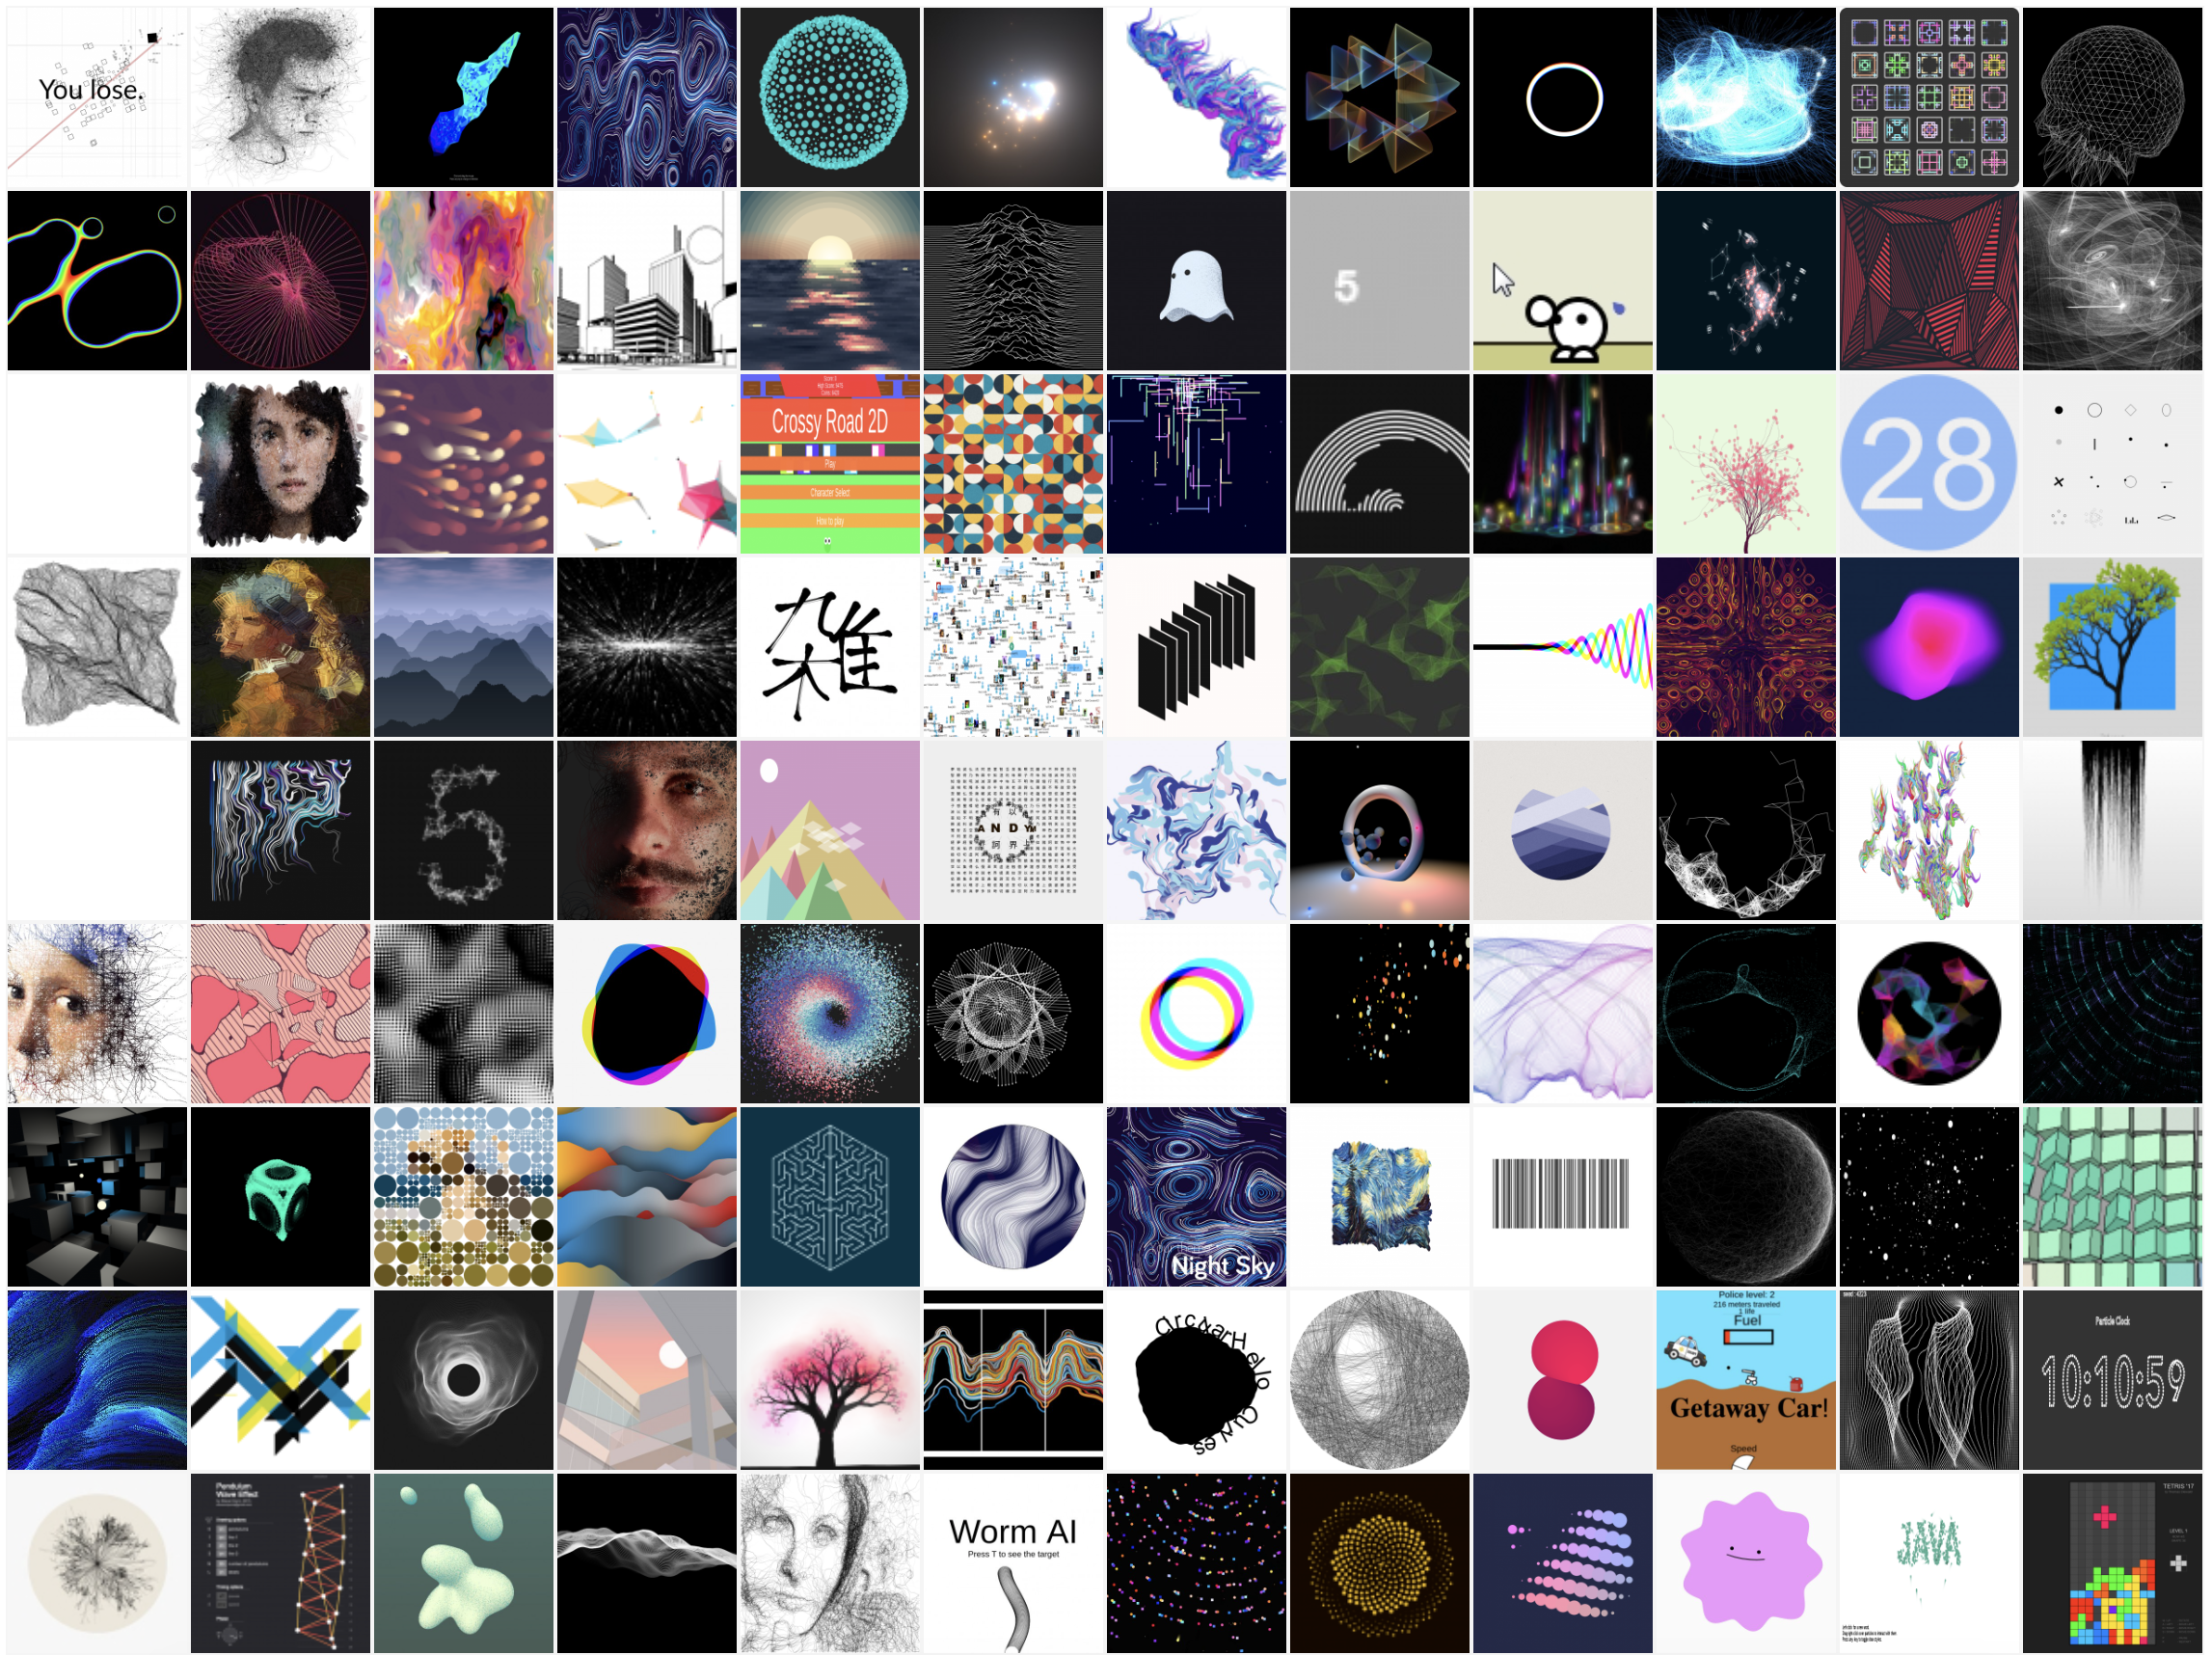
\includegraphics[max width=\textwidth]{images/normative.png}
    \caption[Openprocessing screenshot]{A screenshot of openprocessing.org, depicting  prevalent aesthetic trends}
    \label{fig:normative}
\end{figure}
